\subsection{Funktionsweise} \label{sec:funktionsweise}
Der Dōjō ist eine Art Audioguide, welcher für Museen designt wurde und diverse Funktionen beinhaltet. Abbildung \ref{fig:Funktion Dojo} zeigt den von der Auftraggeberin designten Prototypen. Einer der grössten Unterschiede zu einem herkömmlichen Audioguide ist die Sprachausgabe mittels einem Knochenschallaktor und nicht wie gewöhlich mit einem Lautsprecher. Eine weitere Eigenheit ist der integrierte {\glqq Like\grqq}-Button, mit dem man die entsprechenden Ausstellungsstücke {\glqq liken\grqq} kann. Dadurch lässt sich für jeden Besucher individuell eine persönliche Kunstobjektliste zusammenstellen, die nur noch die entsprechenden Objekte mit einem {\glqq Like\grqq} enthält. Das ermöglicht es, am Ende des Besuchs jeder Person eine Liste mit den jeweiligen Informationen zum Ausstellungsobjekt auszuhändigen. Ansonsten verfügt der Dōjō über die gleichen Funktionen, die man von einem üblichen Audioguide erwarten würde, wie z.B. der Audiowiedergabe, dem Haltemodus oder der Lautstärkeregelung.

\begin{figure}[H]
	\begin{center}
		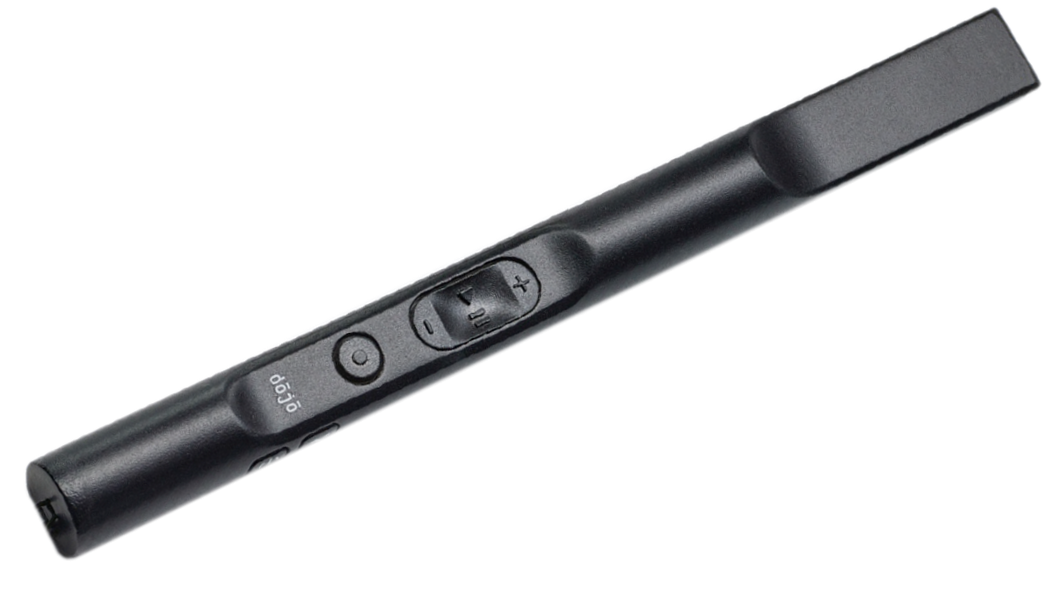
\includegraphics[width=120mm]{data/Dojo.png}
		\caption[Dōjō als Modell]{Dōjō als Modell} %picture caption
		\label{fig:Funktion Dojo}
	\end{center}
\end{figure}

Das Herzstück des Dōjōs ist ein zentraler NRF52-Mikrocontroller von Nordic Semiconductor mit integriertem und low-Energy fähigem Bluetooth-Stack. Die verwendeten Daten werden auf einer SD-Karte gespeichert. Bei Bedarf werden die Audiodateien an den Verstärker weitergegeben und schliesslich über den Knochenschallaktor wiedergegeben. Die Energieversorgung wird mit einer Li-Ion-Batterie sichergestellt, welche über ein induktives Ladesystem versorgt wird. Abbildung \ref{fig:Teilsysteme} zeigt das technische Lösungskonzept im Überblick.

\begin{figure}[H]
	\begin{center}
		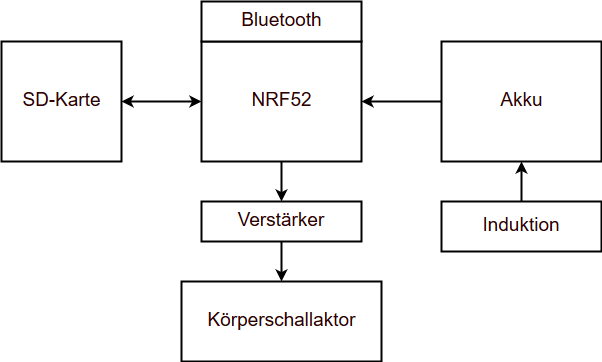
\includegraphics[width=110mm]{data/Loesungskonzept_Teilsysteme.png}
		\caption{Teilsysteme des Dōjōs} %picture caption
		\label{fig:Teilsysteme}
	\end{center}
\end{figure}

Die Funktionen des Dōjōs werden nachfolgend in zwei Bereiche unterteilt. Zuerst wird die Funktionalität aus Sicht des Users beschrieben. Anschliessend werden die relevanten Funktionen aus Sicht der Betreiber erläutert.

Der \textbf{User} geht mit dem Dōjō durch das Museum. Sobald die Bluetooth Beacons genügend nahe sind, erhält der User durch eine aufleuchtende LED ein Signal. Jetzt kann er entscheiden, ob er sich das zugehörige Audio-File anhören will. Trifft dies zu, wird die Audiodatei durch das Betätigen des Play-Buttons abgespielt. Die Lautstärke kann über die Volume-Buttons justiert werden. Falls das Ausstellungsstück dem User gefallen hat, kann die \glqq Like\grqq-Taste gedrückt werden. Dadurch wird das Ausstellungsstück auf einer Liste in der internen SD-Karte gespeichert. Am Ende des Museumsbesuches kann diese Liste ausgewertet werden, wobei die Verwendung dieser Daten nicht Bestandteil der Projektarbeit ist und aus diesem Grund nicht weiterverfolgt wird.

Der \textbf{Betreiber} hat die Aufgabe den Dōjō zu konfigurieren. Dies erfolgt über die dafür vorgesehene SD-Karte, welche mit dem Computer beschrieben wird. Anschliessend kann die Speicherkarte in den Dōjō eingeführt werden. Die Energieversorgung erfolgt über eine induktive Ladestation. Die nächsten beiden Funktionen sind Wunschziele, die vor allem mit Rücksicht auf die Laufzeit realisiert werden. Den Bluetooth-Receiver könnte man kurzzeitig auf ein Bluetooth Beacon umschalten. Der Betreiber müsste nur noch einen Receiver pro Raum installieren. Damit könnte man die gewünschte Lokalisierung der Besucher umsetzen. Das zweite wäre die Möglichkeit per Bluetooth einzelne Audiofiles auf den Dōjō zu übertragen, um im Falle einer Änderung der Ausstellung, die Liste anzupassen und damit aktuell halten zu können.
